\documentclass[xcolor=x11names, compress]{beamer}

%% General document %%%%%%%%%%%%%%%%%%%%%%%%%%%%%%%%%%
\usepackage{graphicx}
\graphicspath{{graphics/}}

\usepackage{tikz}
\usepackage{color}
\input{rgb}

\definecolor{capri}{rgb}{0,.75,1}
\definecolor{coral}{rgb}{1,.2,.2}

\newcommand{\hltyellow}[1]{\colorbox{yellow}{$\displaystyle #1$}}
\newcommand{\hltblue}[1]{\colorbox{capri}{$\displaystyle #1$}}
\newcommand{\hltred}[1]{\colorbox{coral}{$\displaystyle #1$}}
\newcommand{\hltgreen}[1]{\colorbox{green}{$\displaystyle #1$}}

\usepackage{hyperref}

\usepackage{ulem}
\renewcommand<>{\sout}[1]{
  \only#2{\beameroriginal{\sout}{#1}}
  \invisible#2{#1}
}

%%%%%%%%%%%%%%%%%%%%%%%%%%%%%%%%%%%%%%%%%%%%%%%%%%%%%%

%% Beamer Layout %%%%%%%%%%%%%%%%%%%%%%%%%%%%%%%%%%
% \usetheme{Madrid}

\useoutertheme[subsection=false,shadow]{miniframes}
\useinnertheme{default}
\usefonttheme{serif}
\usepackage{palatino}

\setbeamerfont{title like}{shape=\scshape}
\setbeamerfont{frametitle}{shape=\scshape, series = \bfseries}
\setbeamertemplate{frametitle}[default][center]
\setbeamerfont{footnote}{size=\tiny}
\addtobeamertemplate{footnote}{}{\vspace{1ex}} %so that the footnotes do not overlap with navigation symbols at bottom

\setbeamercolor*{lower separation line head}{bg=DeepSkyBlue4} 
\setbeamercolor*{normal text}{fg=black,bg=white} 
\setbeamercolor*{alerted text}{fg=red} 
\setbeamercolor*{example text}{fg=black} 
\setbeamercolor*{structure}{fg=black}
 
\setbeamercolor*{palette tertiary}{fg=black,bg=black!10} 
\setbeamercolor*{palette quaternary}{fg=black,bg=black!10} 

\renewcommand{\(}{\begin{columns}}
\renewcommand{\)}{\end{columns}}
\newcommand{\<}[1]{\begin{column}{#1}}
\renewcommand{\>}{\end{column}}

\def\signed #1{{\leavevmode\unskip\nobreak\hfil\penalty50\hskip2em
  \hbox{}\nobreak\hfil(#1)%
  \parfillskip=0pt \finalhyphendemerits=0 \endgraf}}

\newsavebox\mybox
\newenvironment{aquote}[1]
  {\savebox\mybox{#1}\begin{quote}}
  {\signed{\usebox\mybox}\end{quote}}

%%%%%%%%%%%%%%%%%%%%%%%%%%%%%%%%%%%%%%%%%%%%%%%%%%%%

\begin{document}


%%%%%%%%%%%%%%%%%%%%%%%%%%%%%%%%%%%%%%%%%%%%%%%%%%%%%%
{
  \usebackgroundtemplate{\includegraphics[width=\paperwidth]{back.jpg}}
\begin{frame}[plain]

  \vspace{100pt}
  \title{\bf Selection -- \\Ecological Interaction Networks}

\author{
	Samraat Pawar\\
	\vspace{5pt}
	\url{www.pawarlab.org}\\
	\vspace{5pt}
	{\it  Department of Life Sciences, Silwood Park Campus}\\
Imperial College London\\
  \vspace{5pt}
\today
  % \centering
  % \includegraphics[height = .3.3in]{Imperial_Color1.pdf}
}
 
\titlepage
\date{} 

\end{frame}
}

%%%%%%%%%%%%%%%%%%%%%%%%%%%%%%%%%%%%%%%%%%%%%%%%%%%%%%
\section{\scshape Introduction}
% \subsection{}
%%%%%%%%%%%%%%%%%%%%%%%%%%%%%%%%%%%%%%%%%%%%%%%%%%%%%%

\begin{frame}{Outline}
  \begin{itemize}\setlength{\itemindent}{0em}\itemsep12pt

    \item Introduction

    \item Ecological (Interaction) Networks

    \item Trophic Networks (including Food webs)
    
    % \item Metabolic Basis of Trophic Networks

    \item Summary, Questions, and Readings

  \end{itemize}  

\end{frame}

%%%%%%%%%%%%%%%%%%%%%%%%%%%%%%%%%%%%%%%%%%%%%%%%%%%%%%
\begin{frame}{Darwin's {\it Gedankenexperiment}}

\begin{columns}[c]
  \column{0.75\textwidth}\centering
  \vspace*{\fill} 
  \begin{quote} 
    ...the presence of a feline animal in large numbers in a district 
  might determine, through the intervention first of mice and then of 
  bees, the frequency of certain flowers in that district!\\
    \centering 
    \hfill -- {\small Darwin 1859, ``The origin of species''}
  \end{quote}
  \vspace*{\fill}
  \column{0.25\textwidth}\centering
  \vspace*{\fill} 
  \includegraphics[width=.65\textwidth]{Darwin.jpg}\\
  {\tiny Public Domain, \url{https://commons.wikimedia.org/w/index.php?curid=11264065} \par} 
  \vspace*{\fill}
\end{columns}

\vspace{5pt}
\begin{columns}[c]
  \column{0.35\textwidth}\centering
    \includegraphics[width=\linewidth]{Reef.jpg}
  \column{0.35\textwidth}\centering
    \includegraphics[width=0.94\linewidth]{Rainforest.jpg}
\end{columns}
\vspace{6pt}
\pause 
\begin{itemize}
  \item Complex interaction networks between species' populations underpin ecosystems
\end{itemize}
  
\end{frame}

%%%%%%%%%%%%%%%%%%%%%%%%%%%%%%%%%%%%%%%%%%%%%%%%%%%%%%
\begin{frame}{Objectives}

  \vspace{6pt}
  \begin{itemize}[<+->]\setlength{\itemindent}{0em} \itemsep20pt
      \item We will learn about Ecological Interaction Networks (henceforth, ``Ecological Networks'') in this lecture
      \item We will focus on consumer-resource (AKA {\it Trophic}) interaction-based Ecological Networks (henceforth, ``Trophic Networks''), especially, Food webs 
      
      \item Mutualistic Networks coming up in next lecture
  \end{itemize}
  
\end{frame}

%%%%%%%%%%%%%%%%%%%%%%%%%%%%%%%%%%%%%%%%%%%%%%%%%%%%%%
\section{\scshape Ecological Networks}
%%%%%%%%%%%%%%%%%%%%%%%%%%%%%%%%%%%%%%%%%%%%%%%%%%%%%

%%%%%%%%%%%%%%%%%%%%%%%%%%%%%%%%%%%%%%%%%%%%%%%%%%%%%%
\begin{frame}{Ecological Networks}

\begin{columns}[c]
  \column{0.6\textwidth}
  \begin{itemize}[<+->]\setlength{\itemindent}{0em} \itemsep6pt
    \item {\bf Ecological Network}: Network of interactions where {\it nodes} ($\boldsymbol{\cdot}$) are individuals or (usually, species') populations, and {\it links} (---) the interactions between pairs of nodes 
  \end{itemize}
  \column{0.4\textwidth}\centering
  {\footnotesize The Silwood Park Food web}\\
  \vspace{3pt}
  \includegraphics[width=.7\linewidth]{SilwoodWeb.png}
\end{columns}
\pause 
\vspace{6pt}
\begin{itemize} \setlength{\itemindent}{-1em}
  \item Types:
  \begin{itemize}\setlength{\itemindent}{-2em}
  \item Trophic networks ($+/-$) (e.g., food webs)
  \item Mutualistic networks ($+/+$) (e.g., plant-pollinator networks) -- {\it next lecture}    
  \item Competitive networks ($-/-$) (e.g., plant-plant or microbe-microbe)
  \item Behavioural networks ($+/-$, $+/+$,$+/-$ ) (e.g., social networks)
 \end{itemize} 
\end{itemize}

\end{frame}

%%%%%%%%%%%%%%%%%%%%%%%%%%%%%%%%%%%%%%%%%%%%%%%%%%%%%%
\begin{frame}{Origin of Ecological networks}

  \begin{center}
    
  \begin{tikzpicture}
    \node (img1) {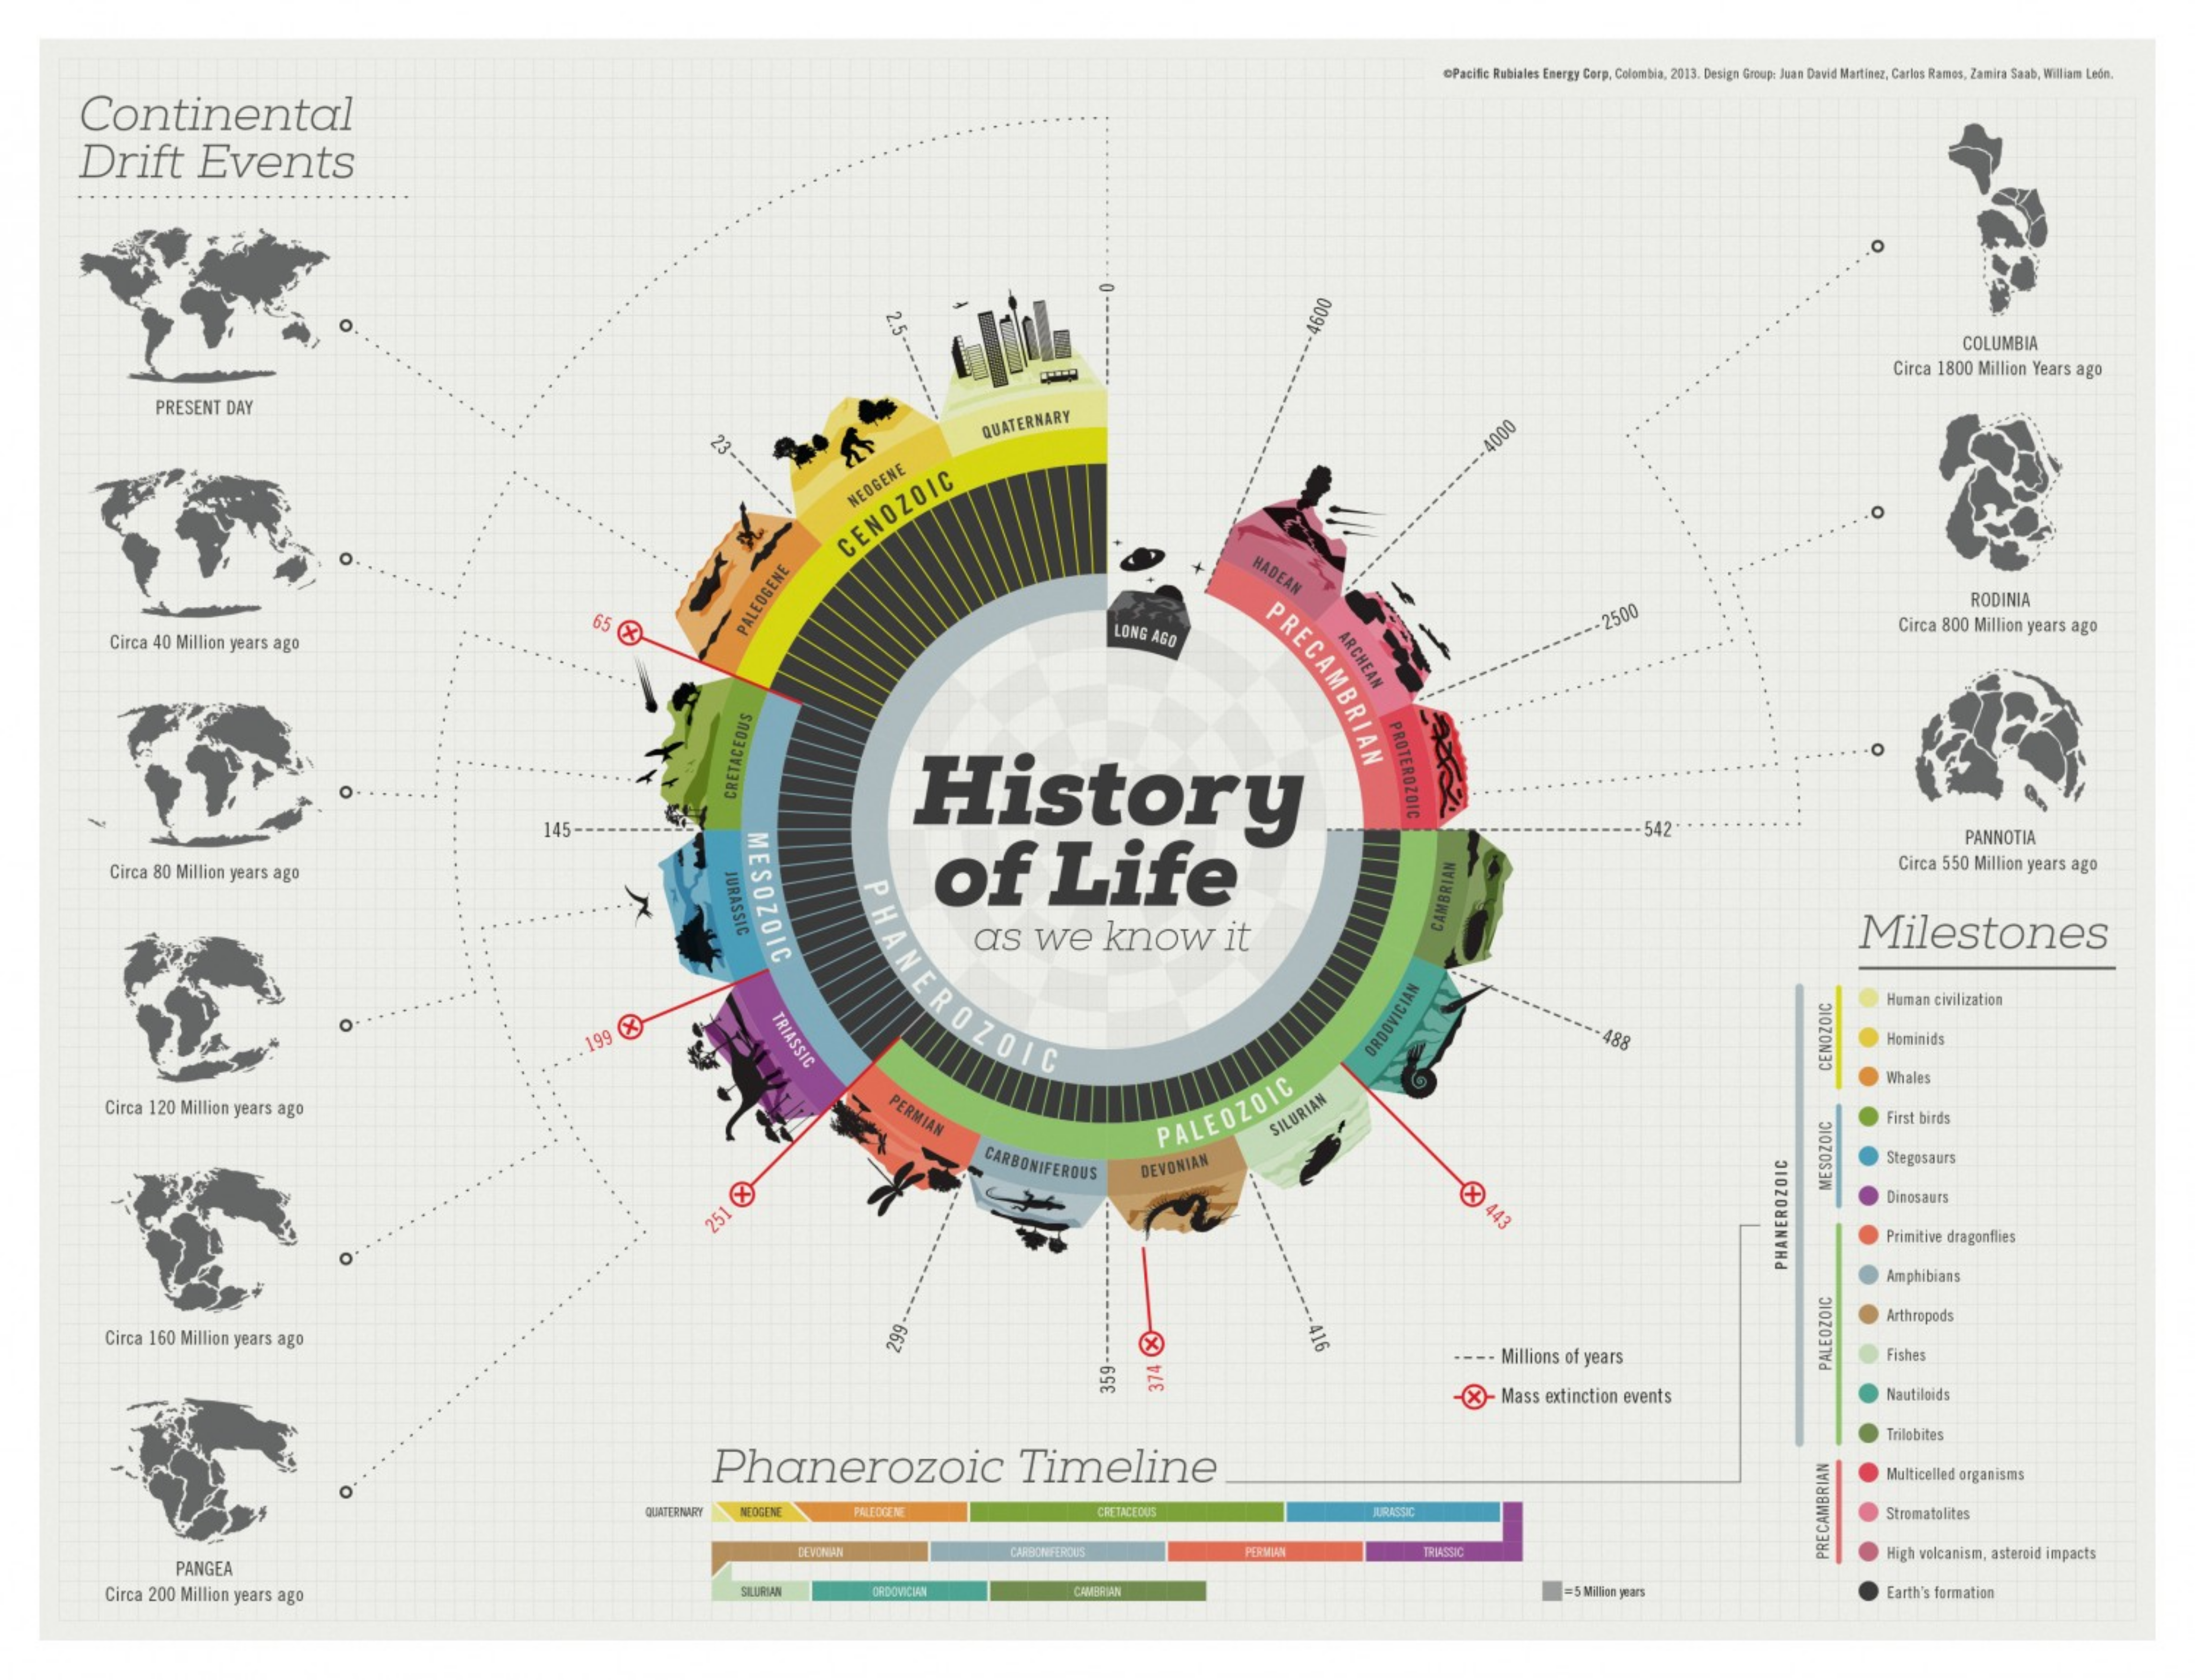
\includegraphics[width=3.3in]{History1.png}};
    \pause
    \node (img2) at (img1) {\includegraphics[width=3.3in]{History2.png}};
    \pause
    \node (img3) at (img1) {\includegraphics[width=3.3in]{History3.png}};
    \pause
    \node (img4) at (img1) {\includegraphics[width=3.3in]{History4.png}};
    \pause
    \node (img5) at (img1) {\includegraphics[width=3.3in]{History5.png}};
  \end{tikzpicture}
  \end{center}
  \vspace{-10pt}
  
  \begin{itemize}
    \item Ecological networks are almost as old as life itself
    \begin{itemize}
      \item \it Ancient microbes had trophic interactions
    \end{itemize}
  \end{itemize}
  
  \end{frame}

%%%%%%%%%%%%%%%%%%%%%%%%%%%%%%%%%%%%%%%%%%%%%%%%%%%%%
\begin{frame}{Why study Ecological Networks?}

  \pause
  
  \begin{columns}[c]
    \column{0.6\linewidth}
      \begin{itemize}[<+->]\setlength{\itemindent}{0em}\itemsep4pt
        \item Species invasions (Trophic networks)
        \item Biodiversity conservation (Trophic  networks)
        \item Harvesting (e.g., fisheries) (Trophic networks)
        \item Ecosystem function (e.g., carbon cycling) (Trophic networks, Competitive networks) 
        \item Pollination services (Mutualistic networks) (next lecture)
        \item Social change (Behavioural networks)
      \end{itemize}
    \column{0.4\linewidth}\centering
    \includegraphics[width=.9\textwidth]{Kudzu.pdf}\\	
    \vspace{6pt}
    \includegraphics[width=.9\textwidth]{Pieter_Fish.jpg}		
  \end{columns}
  
  \end{frame}  

%%%%%%%%%%%%%%%%%%%%%%%%%%%%%%%%%%%%%%%%%%%%%%%%%%%%%%
\begin{frame}{Structure of Ecological networks}

  \begin{itemize}[<+->]
    \item Ecological networks are built from {\it Modules}\footnotemark[1]: groups of few ($>2$) inter-corrected nodes 
    \item The modules that are most commonly seen (at an above-random\footnotemark[2]~frequency) are called {\it Motifs}  
  
    \begin{center}    
      \includegraphics[width=.55\linewidth]{Motifs.pdf}\\
      {\tiny Bascompte \& Stouffer Phil Trans Roy Soc B 2009}
    \end{center}
  
    \item Certain modules may be selected (or de-selected) over time because they increase (or decrease) stability of the network / system (species in them go extinct --- ``species sorting'')
  
  \end{itemize} 
  
  \footnotetext[1]{We will learn about specific Modules in next section on Trophic Networks} 
  
  \only<2->{\footnotetext[2]{Because they have been favoured (selected) by some process; read paper by Borrelli et al TREE 2015}}
  
\end{frame}
  
 %%%%%%%%%%%%%%%%%%%%%%%%%%%%%%%%%%%%%%%%%%%%%%%%%%%%%%
\begin{frame}{Structure and stability of ecological networks}
  
\begin{itemize}[<+->]\itemsep0pt
  
  \item Understanding how {\it structure} (pattern of interconnections) relates to {\it stability} and resilience of Ecological Networks is a (if not {\it the}) ``Holy Grail'' of Ecology
  \begin{itemize}
    \item {\bf Network (or System) Stability}: ability of the system to recover (e.g., not lose any species) from disturbances
    \item   {\bf Network (or System) Resilience}: ability of the system to buffer/absorb disturbances
  \end{itemize}
  \pause
  \begin{columns}[c]
    \column{0.55\linewidth}
      \begin{itemize}[<+->]\setlength{\itemindent}{-1em}\itemsep4pt
        \item A number of structures have been related to stability (e.g., Chain/Path Length, Number of Trophic Levels, Modularity)
        \item There is no single measure of structure that holds the answer
      \end{itemize}
    \column{0.45\linewidth}\centering
    \includegraphics[width=\linewidth]{Network_Structure.pdf}\\
    {\tiny Ho et al Ecology Letters 2021}  
  \end{columns}

\end{itemize} 

\end{frame}
  
%%%%%%%%%%%%%%%%%%%%%%%%%%%%%%%%%%%%%%%%%%%%%%%%%%%%%%
\section{\scshape Trophic Networks}
%%%%%%%%%%%%%%%%%%%%%%%%%%%%%%%%%%%%%%%%%%%%%%%%%%%%%%

%%%%%%%%%%%%%%%%%%%%%%%%%%%%%%%%%%%%%%%%%%%%%%%%%%%%%%
\begin{frame}{Trophic Networks}

\begin{itemize}
  \item {\bf Trophic Networks}: Networks of populations linked by ``who-eats-whom'' or ``who-eats-what'' interactions 
\end{itemize} 

\begin{columns}[c]
  \column{0.6\textwidth}
  \pause
  \begin{itemize}
    \item {\bf Food webs}: ``who-eats-whom'' interactions (animal-eat-animal or animal-eat-plant)   
  \end{itemize}\small
  \centering    
  \includegraphics[width=\linewidth]{FW_DB.png}\\
    \vspace{-6pt}
    {\tiny Ho et al Ecology Letters 2019}
  \column{0.4\textwidth}
  \pause
  \begin{itemize}\small
    \item {\bf Microbial networks}: ``who-eats-what'' interactions of Consumers feeding on organic carbon sources
  \end{itemize}
  \centering
   \includegraphics[width=.9\linewidth]{Bacteria_Net.png}\\
   \vspace{-6pt}
   {\tiny Goldford et al Science 2018}
\end{columns}

\end{frame}
  
%%%%%%%%%%%%%%%%%%%%%%%%%%%%%%%%%%%%%%%%%%%%%%%%%%%%%%
\begin{frame}{Early work on Trophic Networks }
  
\centering
      \includegraphics[width=.7\textwidth]{Camerano_plate-1.pdf} % Camerano 1880 Atti Reale Acc Scienze Torino 1880
  
\end{frame}
  
%%%%%%%%%%%%%%%%%%%%%%%%%%%%%%%%%%%%%%%%%%%%%%%%%%%%%%
  \begin{frame}{Early work on food webs}
      
    \centering
      \includegraphics[width=.8\textwidth]{EltonFW.pdf} %Summerhayes \& Elton 1923 J Ecol    
  
  \end{frame}
  
%%%%%%%%%%%%%%%%%%%%%%%%%%%%%%%%%%%%%%%%%%%%%%%%%%%%%%
\begin{frame}{Modern understanding of Food webs}

  \begin{center}
    \includegraphics[width=.55\textwidth]{Foodweb.pdf}
  \end{center} 
  \vspace{-6pt}
  \begin{itemize}[<+->] \itemsep0pt
    \item Certain structural features can predict  food web stability\footnotemark[1]
    \item Food webs have systematic body size structure (e.g., size increases with trophic level)\footnotemark[2]
    \item There are consistent efficiencies of energy transfer across trophic levels (only $\approx 10-20\%$ per level)
 \end{itemize} 

 \footnotetext[1]{Everything you learned about this in the previous section applies to food webs}
 
 \only<2->{\footnotetext[2]{Review lecture on Energy and Metabolism, and the effect of size on trophic/biomss/ecological pyramids}}
\end{frame}

  %%%%%%%%%%%%%%%%%%%%%%%%%%%%%%%%%%%%%%%%%%%%%%%%%%%%%%
  \begin{frame}{Food web modules}
  
    \begin{itemize}[<+->] \itemsep6pt
       \item Food webs are also made of modules (like other Ecological networks); three key modules are,
       \begin{itemize}
         \item Resource competition (two consumers, one resource)
         \item Apparent competition (two resources, one consumer)
         \item Food chains (one resource and atleast two consumers)
       \end{itemize} 
    \end{itemize}
  
    \pause
    \begin{columns}[c]
      \column{0.3\textwidth}\centering
        \includegraphics[width=.8\textwidth]{logo.pdf}\\
        \includegraphics[width=.8\textwidth]{device.png}
      \column{0.7\textwidth}\centering
        \begin{itemize}[<+->] \itemsep3pt
          \item Play EcoBuilder to understand these modules (and more)
          \item \small \url{https://ecobuildergame.org} (to play in web browser: \url{https://ecobuildergame.org/Beta})
          \item Try out as much of the {\it Learning World} as you can\footnotemark
          \item Think about the role of {\it indirect interactions}, and {\it trophic cascades}
      \end{itemize}
    \end{columns} 

    \only<5->{\footnotetext{Assuming you have already played to Level 4 at least; see preceding lecture on Consumer-Resource Interactions}}

\end{frame}

%%%%%%%%%%%%%%%%%%%%%%%%%%%%%%%%%%%%%%%%%%%%%%%%%%%%%%
\begin{frame}{Metabolic basis of trophic networks}

  \begin{center}
    \includegraphics[width=\textwidth]{Roadmap.pdf}
  \end{center}
\vspace{10pt}
  \begin{itemize}\setlength{\itemindent}{0em} \itemsep4pt
    \item Individual-level metabolism, through species interactions, determines trophic network structure and dynamics
  \end{itemize}

\end{frame}
%%%%%%%%%%%%%%%%%%%%%%%%%%%%%%%%%%%%%%%%%%%%%%%%%%%%%%

\begin{frame}{Metabolic basis of food web dynamics}

\begin{columns}[c]
  \column{0.65\textwidth}
    \begin{itemize}\setlength{\itemindent}{0em} \itemsep4pt
      
    \item The effect of metabolism on network structure and dynamics is mediated by 
    \begin{itemize}\setlength{\itemindent}{-1em}
      \item Body size[1]
      \item Size difference (ratio) between species pairs[1]
      \item Temperature\footnotemark[1] and Nutrients
      \item Spatial dimensionality\footnotemark[1]
    \end{itemize} 

  \end{itemize}
  \column{0.35\textwidth}
    \includegraphics[width=.7\textwidth]{FoodWeb.pdf}
\end{columns}
\pause
\begin{columns}[c]
  \column{0.65\textwidth}
    \begin{itemize}\setlength{\itemindent}{0em} \itemsep4pt
      
      \item These factors also influence community assembly/recovery rate
      
    \end{itemize}
  \column{0.35\textwidth}

  \includegraphics[width=\textwidth]{Assembly_1.pdf}
\end{columns}
\footnotetext[1]{Review lecture on Consumer-Resource interactions}
\end{frame}

  
%%%%%%%%%%%%%%%%%%%%%%%%%%%%%%%%%%%%%%%%%%%%%%%%%%%%%
\begin{frame}{The Final EcoBuilder Challenge}

  \begin{itemize}[<+->] \itemsep6pt
      \item How complex a network can you build?
      \item {\it Who can get the highest score in the class?}
  \end{itemize}

  \begin{columns}[c]
    \column{0.3\textwidth}\centering
      \includegraphics[width=.8\textwidth]{logo.pdf}\\
      \includegraphics[width=\textwidth]{device.png}
    \column{0.7\textwidth}\centering
      \begin{itemize}[<+->] \itemsep8pt
        \item \small \url{https://ecobuildergame.org} (to play in web browser: \url{https://ecobuildergame.org/Beta}
        \item You will have to get through the {\it Learning World} to get to the {\it Research World}
        \item In the {\it Research World}, try and maximize your score!
    \end{itemize}
  \end{columns} 

\end{frame}

%%%%%%%%%%%%%%%%%%%%%%%%%%%%%%%%%%%%%%%%%%%%%%%%%%%%%%
\section{\scshape Summary}
%%%%%%%%%%%%%%%%%%%%%%%%%%%%%%%%%%%%%%%%%%%%%%%%%%%%%%
  \begin{frame}{Summary}
  
    \begin{itemize}[<+->] \setlength{\itemindent}{0em} \itemsep10pt

        \item Darwin's {\it Gedankenexperiment} --- every ecosystem is more than the sum of its parts (species's populations) because of underlying interaction networks
        
        \item Network motifs (small sub-networks) are the building blocks of Ecological networks
        \begin{itemize}
          \item They can be selected/favoured by stability
        \end{itemize} 
    
        \item Trophic networks are arguably the most important type of ecological network
        \begin{itemize}
          \item Important for understanding the many effects of of global change
        \end{itemize}

        \item Metabolism is key for understanding trophic networks and the emergent ecosystem dynamics
        
    \end{itemize}
  
  \end{frame}  

%%%%%%%%%%%%%%%%%%%%%%%%%%%%%%%%%%%%%%%%%%%%%%%%%%%%%%
\begin{frame}{Discussion Questions}

  \begin{enumerate}\setlength{\itemindent}{-2em}\itemsep4pt
  
    \item What sorts of interactions might ancient microbes have had? What type(s) of Ecological Network(s)? 

    \item What are the differences and similarities between microbial networks (who-eats-what type) and food webs (who-eats-whom type)? 

    \item What did you learn about types of building blocks of food webs from the EcoBuilder game? What types of trophic interaction modules?
    
    \item What role do indirect interactions play in trophic network / food web dynamics?

    \item How are trophic/biomass/ecological pyramids related to body size structure in food webs?

    \item How do you think climatic temperature (and warming) affects trophic networks / food webs? 

  \end{enumerate}

\end{frame}

  
  %%%%%%%%%%%%%%%%%%%%%%%%%%%%%%%%%%%%%%%%%%%%%%%%%%%%%%
  \begin{frame}{Readings}
  
  \begin{enumerate}\setlength{\itemindent}{-2em}\itemsep4pt
  
    % \item Milo, R. et al. Network motifs: simple building blocks of complex networks. Science 298, 824--7 (2002).

    \item Bascompte, J. \& Stouffer, D. B. The assembly and disassembly of ecological networks. Philosophical Transactions of the Royal Society (B: Biological Sciences) 364, 1781--1787 (2009).

    \item Borrelli, J. J. et al. Selection on stability across ecological scales. Trends in Ecology and Evolution 30, 417--425 (2015).

    \item Pawar, S., Dell, A. I. \& Savage, V. M. From metabolic constraints on individuals to the dynamics of ecosystems. In: {\it Aquatic Functional Biodiversity: An Ecological and Evolutionary Perspective}, 3--36 (Academic Press, 2015).
    
    % \item Woodward, G. et al. Body size in ecological networks. Trends in Ecology and Evolution 20, 402--9 (2005).
    
    % \item Ho H. C., Tylianakis, J. M. \& Pawar, S. Predation risk influences food-web structure by constraining species diet choice. Ecology Letters 22, 1734--1745 (2019).
    
    \item Ho, H. C., Tylianakis, J. M. \& Pawar, S. Behaviour moderates the impacts of food-web structure on species coexistence. Ecology Letters 24, 298--309 (2021).
    
    \item Goldford, J. E. et al. Emergent simplicity in microbial community assembly. Science 361, 469--474 (2018).

\end{enumerate}
  
\end{frame}

\end{document}